\begin{figure}[h!]
\begin{center}
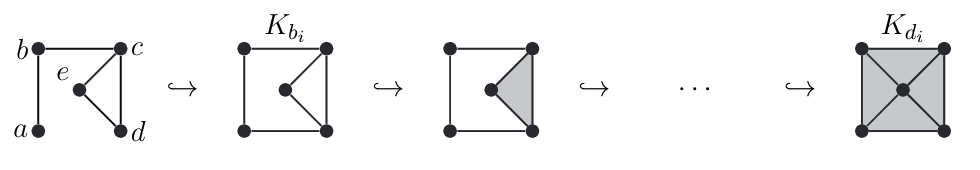
\includegraphics[width=1\textwidth]{figures/volumeexample.jpg}% This is a *.eps file
\end{center}
\caption{A situation in which a volume-optimal cycle is different from the uniform minimal cycle. Consider the filtered simplicial complex pictured. For the persistence interval $[b_i,d_i)$, the cycle with minimal $0$-norm (fewest number of edges) is $(a,b) + (b,c) + (c,d)  + (d,a)$.
However, the volume-optimal cycle would be found as follows: considering $K_{d_i}$, we must find the fewest $2$-simplices whose boundary captures the persistence interval. In this case, we would have an optimal volume $(a,b,e) + (b,c,e) + (a,d,e)$ and volume-optimal cycle $(a,b) + (b,c) + (c,e) + (e,d) + (d,a)$. 
}\label{fig:volumeoptimal}
\end{figure}